\documentclass[10pt,letterpaper]{article}

\usepackage[top=2cm,right=2cm,bottom=2cm,left=2cm,nohead,nofoot]{geometry}

\usepackage{amsmath}
\usepackage{graphicx}
\usepackage{indentfirst}
\usepackage{url}
\usepackage{mdwlist}
\usepackage[compact]{titlesec}
\usepackage[T1]{fontenc}
\usepackage{palatino}
\usepackage[brazil]{babel}
\usepackage[utf8]{inputenc}
\usepackage{enumerate}

\pagestyle{empty}
\setcounter{secnumdepth}{5}

\makeatletter
\def\thickhrulefill{\leavevmode \leaders \hrule height 1pt\hfill \kern \z@}
\renewcommand{\maketitle}{
	\begingroup
		\parindent \z@
		\begin{center}
			{\normalsize \@author\par}%
			\thickhrulefill\par
			{\small\raggedleft \@date\par}%
			{\Large\raggedright \@title\par}%
		\end{center}%
	\endgroup
}
\makeatother

\title{F 429: Experimento II}
\author{033910 Leandro Mendes | 104198 Thiago Verratti | 118451 Rafael Mendes | 121096 Leonardo Sorensen}
\begin{document}
\maketitle
\tableofcontents
\listoffigures
\listoftables
\newpage
\section{Introdução}
Este experimento propõe-se a estudar as experimentalmente e analizar as formas de onda dos circuitos integrador e
diferenciador. Neste caso, são do tipo RC e compostos por uma fonte, um resistor e um
capacitor ligados em série.\\
Analisamos também transientes em circuito ressonante série RLC. Os transientes podem ser estudados no laboratório excitando o circuito com uma onda quadrada de período muito maior que a constante de tempo do circuito.
\section{Metodologia}
\subsection{Instrumentos e Componentes}
Os instrumentos e componentes utilizados estão listados abaixo com seus respectivos valores nominais.
\begin{itemize}
\item{Gerador de Funções Tektronix CFG 253.} 
\item{Osciloscópio digital Tektronix TDS1000.}
\item{Resistências nominais de 47$\Omega$ e 150$\Omega$.}
\item{Resistência de décadas (10$\Omega$ a 10K$\Omega$).}
\item{Capacitor de 0.22$\mu$F.}
\item{Indutor de 50mH.}
\end{itemize}
\subsubsection{Medidas}
\begin{enumerate}[(a)]
\item \textbf{Impedância interna do gerador}: Para determinar a impedância interna do gerador de funções, começamos com a aproximação de que esta é puramente resistiva e independe da frequência, modo de onda ou corrente que fornece. Feita essa hipótese, podemos encontrar a resistência interna $R_G$ do gerador montando o circuito como na figura abaixo. 
  \begin{figure}[!htb]
    \centering
    \label{impger}
    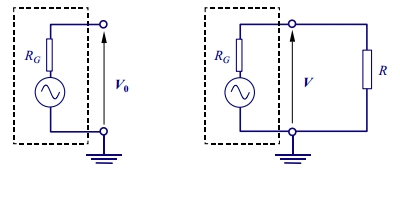
\includegraphics[scale=0.5]{impger.jpg}
    \caption{Circuito representativo para medida da resistência interna do gerador}
  \end{figure}
Primeiro medimos a tensão de saída do gerador de funções conectando-o diretamente ao osciloscópio. Medida a tensão de pico $V_0$, colocamos agora um resistor em paralelo ao circuito, e obtemos um valor para V. Com essas medidas podemos encontrar um valor para $R_G$, já que sabendo que \boxed{V = RI}
\end{enumerate}
\end{document}


